\documentclass[11pt,a4paper]{article}

% ── Layout ────────────────────────────────────────────────────────
\usepackage[a4paper,margin=2.35cm]{geometry}
\usepackage{setspace}
\setstretch{1.10}

% ── Encoding & language ───────────────────────────────────────────
\usepackage[utf8]{inputenc}
\usepackage[T1]{fontenc}
\usepackage[english]{babel}
\usepackage{microtype}

% ── Font: Helvetica (sans-serif) ──────────────────────────────────
\usepackage[scaled=0.95]{helvet}
\renewcommand{\familydefault}{\sfdefault}

% ── Colour palette ────────────────────────────────────────────────
\usepackage[table,xcdraw]{xcolor}
\definecolor{novagreen}{RGB}{100,155,0}
\definecolor{darkgray}{RGB}{60,60,60}
\definecolor{lightgray}{RGB}{245,245,245}

% ── Headers / footers ─────────────────────────────────────────────
\usepackage{fancyhdr}
\pagestyle{fancy}
\fancyhf{}
\fancyhead[L]{\footnotesize\textcolor{darkgray}{RL for Sepsis Treatment --- ICU-Sepsis}}
\fancyhead[R]{\footnotesize\textcolor{darkgray}{NOVA IMS $\cdot$ Reinforcement Learning 2025/2026}}
\fancyfoot[C]{\footnotesize\thepage}
\renewcommand{\headrulewidth}{0.4pt}
\renewcommand{\footrulewidth}{0pt}

% ── Section styling (novagreen) ───────────────────────────────────
\usepackage{titlesec}
\titleformat{\section}{\bfseries\color{novagreen}}{\thesection}{0.8em}{}
\titleformat{\subsection}{\color{novagreen}}{\thesubsection}{0.8em}{}
\titleformat{\subsubsection}{\bfseries\color{darkgray}}{\thesubsubsection}{0.8em}{}
\titlespacing*{\section}{0pt}{8pt}{4pt}
\titlespacing*{\subsection}{0pt}{6pt}{3pt}
\titlespacing*{\subsubsection}{0pt}{4pt}{2pt}

% ── Math, graphics, floats ────────────────────────────────────────
\usepackage{amsmath, amssymb}
\usepackage{graphicx}
\usepackage{float}
\usepackage{placeins}
\graphicspath{{figures/}{../plots/}{plots/}{./}}

% ── Tables ────────────────────────────────────────────────────────
\usepackage{booktabs}
\usepackage{multirow}
\usepackage{array}
\usepackage{tabularx}
\usepackage{colortbl}
\newcommand{\tH}[1]{\textcolor{novagreen}{\textbf{#1}}}
\newcommand{\gmid}{\arrayrulecolor{novagreen}\midrule\arrayrulecolor{black}}

% ── Captions ──────────────────────────────────────────────────────
\usepackage{caption}
\captionsetup{font=small, labelfont={bf,color=novagreen}, skip=4pt}

% ── Lists ─────────────────────────────────────────────────────────
\usepackage{enumitem}
\setlist[itemize]{noitemsep, topsep=2pt, parsep=0pt, partopsep=0pt,
                  leftmargin=1.4em, label=\textcolor{novagreen}{\textbullet}}

% ── Paragraph spacing ─────────────────────────────────────────────
\setlength{\parindent}{0pt}
\setlength{\parskip}{2pt}

% ── Hyperlinks ────────────────────────────────────────────────────
\usepackage[colorlinks=true, linkcolor=novagreen, citecolor=darkgray,
            urlcolor=novagreen, pdfborder={0 0 0}]{hyperref}

\begin{document}

% ============================================================
% TITLE PAGE
% ============================================================
\begin{titlepage}
\thispagestyle{empty}
\centering
\vspace*{0.8cm}
{\small\color{darkgray} Master's in Data Science \& Advanced Analytics}\\[2pt]
{\small\color{darkgray} Reinforcement Learning $\cdot$ 2025/2026}
\vspace{0.8cm}

{\color{novagreen}\rule{\linewidth}{2pt}}\\[10pt]
{\LARGE\bfseries\color{darkgray} Reinforcement Learning for\\[6pt]
Sepsis Treatment Optimisation in the ICU}\\[10pt]
{\large\color{darkgray} Tabular and Deep Policies on the \textit{ICU-Sepsis} Benchmark}\\[10pt]
{\color{novagreen}\rule{\linewidth}{2pt}}

\vspace{0.8cm}
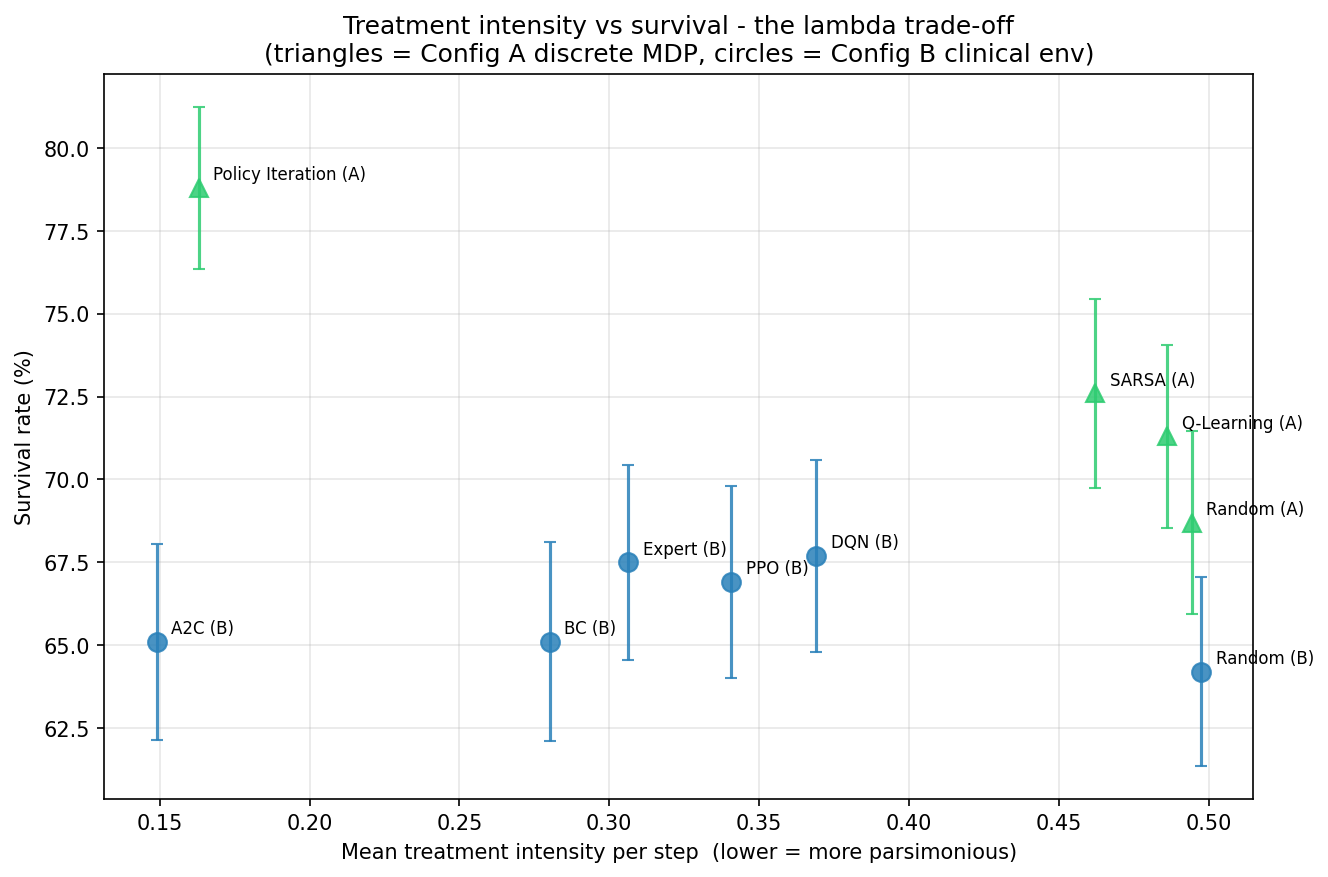
\includegraphics[width=0.74\textwidth]{configAB_pareto.png}
\vspace{0.6cm}

{\small\bfseries\color{darkgray} GROUP}\\[0.8em]
{\small\color{darkgray}
  \begin{tabular}{ll}
    Gonçalo Gomes Arrobas        & 20250421 \\[4pt]
    Maria Tavares Pimentel       & 20250466 \\[4pt]
    Tiago Stubner Lucas Antunes  & 20250357 \\[4pt]
  \end{tabular}
}
\vfill
{\small\color{darkgray} Source code:
\href{https://github.com/mariatavarespimentel/RL-ICU-Sepsis}{github.com/mariatavarespimentel/RL-ICU-Sepsis}}\\[8pt]
{\small\color{darkgray} NOVA Information Management School (NOVA IMS)}\\[4pt]
{\small\color{darkgray} June 2026}
\vspace{0.4cm}\\
{\color{novagreen}\rule{\linewidth}{1pt}}
\end{titlepage}

\tableofcontents
\thispagestyle{empty}
\newpage
\setcounter{page}{1}


% ============================================================
\section{Executive Summary}

We learn ICU treatment policies for sepsis on the \textit{ICU-Sepsis-v2}
benchmark \cite{choudhary2024}, derived from MIMIC-III through the AI~Clinician
pipeline \cite{komorowski2018}. Each episode is one patient trajectory; at every
step the agent chooses a combined vasopressor and intravenous-fluid dose, and the
episode ends in survival ($+1$) or death ($0$), with a small per-step
treatment-intensity penalty ($\lambda=0.02$) encoding clinical parsimony. The
benchmark is configured to a deliberately sick cohort (SOFA-biased initial states,
mean start SOFA $\approx 9.0$). Two settings are studied: \textbf{Configuration~A},
a known discrete MDP ($716$ states, $25$ actions), and \textbf{Configuration~B},
a continuous $47$-dimensional clinical environment with three deployment-style
failure modes (episodic observation noise, missing laboratory values, and rare
acute events).

In Configuration~A, \textbf{Policy Iteration} solves the exact MDP and reaches
$\mathbf{78.8\%}$ survival at the lowest treatment intensity ($0.16$); the
model-free agents \textbf{Q-Learning} ($71.3\%$) and \textbf{SARSA} ($72.6\%$)
beat the random baseline ($68.7\%$) but trail the model-based optimum, exactly as
the theory of dynamic programming versus temporal-difference control predicts. In
Configuration~B, \textbf{DQN}, \textbf{PPO} and \textbf{A2C} (with observation
normalisation, SOFA reward shaping and tuned hyperparameters) match the clinician
expert policy on overall survival ($\text{DQN}=67.7\%$, expert $=67.5\%$, random
$=64.2\%$) and exceed it on clean episodes ($\approx 74\%$ vs $71\%$). Across three
training seeds the agents are stable (DQN $65.8\pm1.0\%$, PPO $66.1\pm0.4\%$ at
$300$k steps). Diagnostically, the DQN value estimates show a clear positive
overestimation bias ($+0.194$), the textbook motivation for Double DQN.

A key honest finding, supported by an intensity--survival Pareto analysis, is that
under the sparse reward the agents primarily learn \emph{parsimony} rather than
better survival; reward shaping is what lifts them to expert-level survival. All
results use fixed evaluation seeds, deterministic policies and bootstrap $95\%$
confidence intervals, and we explicitly avoid the off-policy-evaluation pitfalls
highlighted for clinical RL \cite{gottesman2019}.


% ============================================================
\section{Introduction and Problem Formalisation}

Sepsis is a life-threatening response to infection and a leading cause of ICU
mortality. Its treatment is a sequential decision problem under uncertainty with
\emph{delayed consequences}: a dose given now may only reveal its benefit or harm
several hours later. This makes it a natural Reinforcement Learning (RL) problem,
in which an agent learns a policy by interacting with an environment and receiving
a scalar reward \cite{sutton2018}.

\subsection{Markov Decision Process}
The environment is a Markov Decision Process $(\mathcal{S},\mathcal{A},P,R,\gamma)$.
The return is $G_t=\sum_{k\ge 0}\gamma^k R_{t+k+1}$, and the action-value of a
policy $\pi$ is $Q_\pi(s,a)=\mathbb{E}_\pi[G_t\mid S_t=s,A_t=a]$. Following the
ICU-Sepsis convention we use $\gamma=1.0$: episodes are short (about ten steps) and
the objective is the survival probability over the whole trajectory, so time
discounting is neither needed nor desired.

\textbf{Actions.} The action space is $\mathrm{Discrete}(25)$, encoding five
vasopressor levels $\times$ five IV-fluid levels:
$a = 5\cdot v + f$ with $v,f\in\{0,\dots,4\}$ (none, low, medium, high, very high).
The normalised treatment intensity is $\mathrm{INT}(a)=(v+f)/8\in[0,1]$.

\textbf{Reward.} The native reward is sparse: $+1$ on survival, $0$ on death, $0$
on every intermediate step. The benchmark configuration subtracts a small
treatment-intensity penalty $\lambda\cdot\mathrm{INT}(a)$ at each step
($\lambda=0.02$), encoding the clinical preference for parsimonious care, and biases
the initial-state distribution toward sicker patients (mean start SOFA $\approx9.0$),
which makes the task harder and more realistic.

\subsection{The two configurations}
\textbf{Configuration~A (discrete, known MDP).} The observation is an integer
state in $\{0,\dots,715\}$ ($714$ clinical states $+$ two terminal states). The full
transition tensor $P\in\mathbb{R}^{716\times25\times716}$ and reward matrix are
available, so model-based planning is possible; the $Q$-table has only
$716\times25=17{,}900$ entries, making tabular methods feasible.

\textbf{Configuration~B (continuous, clinical).} The observation is the
$47$-dimensional vector of normalised physiological features (SOFA, lactate, mean
arterial pressure, creatinine, heart rate, etc.) for the underlying state. The
dynamics are identical, but tabular methods are no longer applicable and function
approximation is required. Three orthogonal failure-mode wrappers reproduce
deployment challenges discussed for clinical AI \cite{gottesman2019}: episodic
observation noise (probability $0.15$, Gaussian $\sigma=0.10$), episodic missing
laboratory values (probability $0.15$, four features zeroed), and rare acute
events (probability $0.01$ per step, an irreversible death independent of
treatment).

\subsection{How this report answers the brief}
The project statement asks for more than a leaderboard. It asks us to understand
the environment, implement appropriate RL algorithms for each configuration,
compare them fairly, and add a creative extension that is clinically meaningful.
We therefore structure the work around four explicit requirements.

\begin{table}[H]
\centering
\begin{tabularx}{\textwidth}{>{\raggedright\arraybackslash}p{0.27\textwidth}X}
\toprule
\tH{Brief requirement} & \tH{Our response} \\
\gmid
Explore the environment &
We inspect the state/action spaces, reward sparsity, treatment-intensity penalty,
terminal survival signal, SOFA-biased start distribution and the three
Configuration~B failure modes before choosing algorithms. \\
Implement classical RL in Config~A &
We use Policy Iteration because the full model is exposed, and Q-Learning/SARSA as
model-free TD comparators on the same discrete MDP. \\
Move to continuous clinical RL in Config~B &
We keep the same 25 treatment actions but replace the tabular state with a
47-feature clinical observation, requiring DQN, PPO and A2C with observation
normalisation and careful evaluation under corrupted observations. \\
Go beyond the baseline &
We add reward shaping, learning from demonstrations, robustness analysis,
interpretability, overestimation diagnostics and an intensity--survival Pareto
reading, all evaluated on the original unshaped environment. \\
\bottomrule
\end{tabularx}
\caption{Traceability from the project brief to the report contributions.}
\label{tab:brief_trace}
\end{table}

This traceability is important for the final interpretation. A high return alone
is not enough: because the reward contains both survival and an accumulated
treatment penalty, a policy can improve return by treating less without saving
more patients. For that reason, every result below separates \emph{survival},
\emph{return} and \emph{treatment intensity}, and the clinical conclusion is based
on the three together rather than on a single scalar score.


% ============================================================
\section{Methodology}

\subsection{Design principles}
Our methodological choices follow directly from the environment exploration in
the starter notebooks. First, we treat Configuration~A and Configuration~B as
different observation regimes over the same clinical decision idea, not as two
unrelated tasks. Both use the same 25 treatment actions and the same survival
objective, so differences in performance can be interpreted as differences caused
by model access, observation representation and deployment noise.

Second, we always decompose the reward into its two clinical components. The
terminal survival reward is the primary medical outcome; the per-step
$\lambda\mathrm{INT}(a)$ term is a parsimony regulariser that discourages
unnecessarily aggressive dosing. Optimising the summed return without reporting
survival and intensity separately would hide whether an agent is genuinely
improving outcomes or simply exploiting the dense penalty. This is especially
important in Configuration~B, where the survival signal is sparse and noisy.

Third, we use the strongest method that is justified by the information available.
In Configuration~A the transition and reward tensors are known, so an exact
dynamic-programming solution is not only allowed but expected. In
Configuration~B the agent receives only continuous clinical observations and
sampled transitions, so the right comparison is between deep value-based and
actor-critic methods. This prevents an unfair comparison in which a planning
algorithm is used in a setting where the model is unavailable.

\subsection{Configuration~A: tabular algorithms}
We implement the three tabular methods taught in the dynamic-programming and
temporal-difference lectures \cite{sutton2018}.

\textbf{Policy Iteration (model-based).} Alternates policy evaluation,
$V(s)\leftarrow\sum_{s'}P(s'\mid s,\pi(s))[R+\gamma V(s')]$, with greedy policy
improvement until the policy is stable. With $P$ and $R$ available it solves the
Bellman optimality equations exactly and serves as the model-based ceiling. The
policy-evaluation tolerance is set tightly ($\theta=10^{-9}$ in the final run) so
that any difference between Policy Iteration and the learning agents is due to
sample-based learning rather than numerical looseness. Terminal states are treated
as absorbing, so the value of survival/death propagates backward through the
patient trajectory.

\textbf{Q-Learning (off-policy TD).}
$Q(s,a)\leftarrow Q(s,a)+\alpha[r+\gamma\max_{a'}Q(s',a')-Q(s,a)]$, learning the
greedy target policy from $\varepsilon$-greedy behaviour. It is included because it
is the canonical model-free route to the optimal action-value function when the
agent must learn from interaction. In this sparse-reward sepsis task, the max
target is also a useful stress test: if the sampled values are noisy, Q-Learning
can become overconfident in actions that happened to lead to survival in early
episodes.

\textbf{SARSA (on-policy TD).}
$Q(s,a)\leftarrow Q(s,a)+\alpha[r+\gamma Q(s',a')-Q(s,a)]$, bootstrapping through
the action actually taken, hence more conservative under exploration. Because the
reward is sparse and the cohort difficult, both model-free agents use
\emph{optimistic initialisation} ($Q_0=1$, the maximum achievable return) to drive
systematic exploration, trained for $50{,}000$ episodes with $\varepsilon$ annealed
from $1.0$ to $0.01$ over $35{,}000$ episodes ($\alpha=0.1$). The slower annealing
was chosen after the initial notebook run showed that short exploration budgets
leave many clinically relevant state--action pairs under-sampled. SARSA is
therefore not expected to beat Policy Iteration; its role is to show how an
on-policy learner behaves when the behaviour policy itself is exploratory and
clinically costly.

\subsection{Configuration~B: deep reinforcement learning}
The continuous observation and discrete action space lead naturally to the
discrete-action deep methods from the function-approximation and policy-gradient
lectures, implemented with Stable-Baselines3.

\textbf{DQN} \cite{mnih2015}: value-based, off-policy, with experience replay and a
target network; the deep continuation of Q-Learning.
\textbf{PPO} \cite{schulman2017}: on-policy actor-critic with a clipped surrogate
objective.
\textbf{A2C} \cite{mnih2016}: on-policy actor-critic without clipping, a useful
ablation against PPO. Each agent is trained both on raw observations (v1) and with
\texttt{VecNormalize} observation normalisation (v2); since the $47$ features span
very different scales, normalisation is the single largest lever, so v2 is used for
all main results.

The three algorithms cover complementary assumptions. DQN is sample efficient and
well matched to a discrete action space, but it learns a value for every action and
is exposed to overestimation through the max operator. PPO optimises the policy
directly and limits destructive updates through clipping, which is attractive in a
noisy clinical simulator where large policy jumps can collapse performance. A2C is
included as the simpler actor-critic baseline: if PPO only improves because of the
clipped objective, A2C should reveal that; if A2C performs similarly, then the
dominant issue is likely representation/reward rather than the policy-gradient
stabiliser.

The final report run uses $1$M timesteps, the best short-budget Optuna parameters,
and SOFA potential-based reward shaping during training. These are training
interventions only. At evaluation time we reload the learned policy and run it on
the default \texttt{make\_clinical\_env()} reward, without shaping and without
changing failure-mode probabilities. This separation is deliberate: shaping is
allowed to make learning easier, but the reported survival rate must remain the
survival rate on the original project environment.

\subsection{Evaluation protocol}
\label{sec:eval}
All reported numbers use a \emph{fixed} evaluation protocol: a held-out list of
$1{,}000$ evaluation seeds, deterministic action selection, and the default
environment (no shaping, no wrapper changes). Survival is read from the terminal
reward, which is robust to the accumulated intensity penalty and identical across
both configurations. Every metric is reported with a bootstrap $95\%$ confidence
interval. For Configuration~B we additionally bucket each episode by failure mode
(Clean / Noisy / Missing / Acute) using the wrappers' \texttt{info} flags, scoring
all policies on the \emph{same} patients. We evaluate by Monte-Carlo rollout in the
simulator, which sidesteps the off-policy-evaluation difficulties that
\cite{gottesman2019} identify as the central weakness of clinical RL on logged data.

The evaluation is intentionally deterministic even for stochastic training
algorithms. During training, exploration and stochastic gradient updates are
necessary; during evaluation, however, the question is what treatment policy would
be deployed for a given patient state. We therefore use greedy DQN actions and the
deterministic action mode for PPO/A2C. The same seed list is shared across random,
expert, imitation and learned policies, so per-policy differences are not caused by
seeing easier or harder patients.


% ============================================================
\section{Experimental Setup}

Table~\ref{tab:setup} summarises the experiments. Calibration uses $1{,}000$
evaluation episodes per policy; the deep agents use a fast $150$k-step preview in
the notebook and a report-quality $1$M-step run for the headline numbers, plus a
multi-seed reliability study.

\begin{table}[H]
\centering
\begin{tabular}{llccc}
\toprule
\tH{Experiment} & \tH{Config} & \tH{Method(s)} & \tH{Train budget} & \tH{Eval} \\
\gmid
Tabular control       & A & PI, Q-Learning, SARSA   & 50k ep         & 1000 ep \\
Warm-start (LfD)      & A & Q-Learning $\pm$ demos   & 15k ep         & 1000 ep \\
Deep RL (preview)     & B & DQN, PPO, A2C (v1/v2)    & 150k steps     & 1000 ep \\
Deep RL (report)      & B & DQN, PPO, A2C           & 1M steps       & 1000 ep \\
Hyperparameter search & B & DQN, PPO, A2C (Optuna)   & 50k$\times$15  & --- \\
Reward shaping        & B & PPO $\pm$ SOFA shaping   & 1M steps       & 1000 ep \\
Behavioural cloning   & B & MLP on 47-dim obs        & 36k samples    & 1000 ep \\
Multi-seed reliability& B & DQN, PPO ($3$ seeds)     & 300k steps     & 1000 ep \\
\bottomrule
\end{tabular}
\caption{Experimental configuration summary.}
\label{tab:setup}
\end{table}

The random baseline (uniformly random actions) is the performance floor that every
trained policy must beat. As a clinically grounded upper reference we also evaluate
the benchmark's \emph{expert} policy --- the AI~Clinician behaviour policy
\cite{komorowski2018} --- under the same protocol.

The result files are generated in a one-way pipeline. Configuration~A writes
\texttt{configA\_results.json}; the Configuration~B notebook and report scripts
then read that file for the cross-configuration comparison, avoiding hand-copied
numbers. The $1$M deep-RL run writes \texttt{configB\_1m\_results.json} and
\texttt{configB\_1m\_compare\_configs.csv}; the multi-seed and overestimation
checks write separate JSON files. This is a small but important reproducibility
choice: tables in the report are traceable to committed outputs rather than to
manually edited notebook cells.

Table~\ref{tab:metrics} defines the four metrics used throughout. We keep all four
because each answers a different question. Survival answers the clinical question,
return answers the formal RL objective, intensity answers whether the policy is
parsimonious, and failure-mode survival answers whether the policy is robust to
the specific deployment problems introduced by the brief.

\begin{table}[H]
\centering
\begin{tabularx}{\textwidth}{>{\raggedright\arraybackslash}p{0.22\textwidth}X}
\toprule
\tH{Metric} & \tH{Reason for reporting it} \\
\gmid
Survival rate & Primary clinical outcome; computed from terminal survival/death,
not from the penalised accumulated return. \\
Mean return & The actual RL optimisation objective, including the terminal reward
and the treatment-intensity penalty. \\
Mean intensity & Average normalised vasopressor/fluid dose; reveals whether a
policy is clinically parsimonious or simply avoids treatment. \\
Failure-mode buckets & Clean, noisy, missing-lab and acute episodes isolate which
deployment perturbation is responsible for degradation. \\
\bottomrule
\end{tabularx}
\caption{Evaluation metrics and why each is necessary.}
\label{tab:metrics}
\end{table}

For the deep agents, the preview runs are used only for diagnosis and figure
generation during development. The headline table uses the report-quality run:
$1$M timesteps, observation normalisation, tuned hyperparameters and training-only
SOFA shaping. The Optuna search is deliberately treated as a proxy search rather
than a definitive global optimum, because each trial uses only $50$k steps; it
finds sensible learning-rate and entropy/update settings, but the final claims
come from the longer retraining and the fixed evaluation protocol.


% ============================================================
\section{Results: Configuration~A}
\label{sec:resA}

Table~\ref{tab:configA} reports the tabular agents over $1{,}000$ fixed-seed
episodes. The honest and most instructive finding is that the \emph{model-based}
method dominates the \emph{model-free} ones.

\begin{table}[H]
\centering
\begin{tabular}{lcccc}
\toprule
\tH{Algorithm} & \tH{Type} & \tH{Survival} & \tH{Return} & \tH{Intensity} \\
\gmid
Random            & ---                  & $68.7\pm2.8\%$ & $0.588$ & $0.494$ \\
Q-Learning        & model-free off-policy& $71.3\pm2.8\%$ & $0.612$ & $0.486$ \\
SARSA             & model-free on-policy & $72.6\pm2.9\%$ & $0.631$ & $0.462$ \\
\textbf{Policy Iteration} & model-based DP & $\mathbf{78.8\pm2.5\%}$ & $\mathbf{0.751}$ & $\mathbf{0.163}$ \\
\bottomrule
\end{tabular}
\caption{Configuration~A: survival, return and mean treatment intensity ($\pm$
bootstrap $95\%$ CI), $1{,}000$ episodes.}
\label{tab:configA}
\end{table}

Policy Iteration reaches the highest survival ($+10.1$ percentage points over
random) \emph{and} learns the most parsimonious policy (intensity $0.163$ versus
$0.494$ for random): with the exact model it immediately exploits the $\lambda$
penalty structure. Q-Learning and SARSA improve over random but trail the exact
optimum by $\sim6$--$7$ points. This is expected from theory rather than a defect:
the reward is sparse, the cohort difficult, and $17{,}900$ state--action pairs must
be estimated from sampled experience alone. The takeaway is the dynamic-programming
versus temporal-difference lesson made concrete --- \emph{when the model is known,
plan with it}; model-free TD is the right tool only when the model is unavailable,
which is precisely the premise of Configuration~B. Convergence curves, the
survival/intensity bar charts and the per-policy action distributions are given in
Appendix figures \ref{fig:a_learning}--\ref{fig:a_actions}.

The difference between SARSA and Q-Learning is also clinically interpretable.
Q-Learning evaluates the greedy policy even while the behaviour policy is still
exploring, so its update can assign high value to actions that would not be taken
consistently during training. SARSA instead learns the value of the exploratory
policy it actually follows; under a treatment-penalty reward this tends to be more
conservative. That pattern appears in the final metrics: SARSA has slightly higher
survival than Q-Learning and lower intensity, although both remain far from the
planning optimum.

The environment-exploration plots support this reading. Random rollouts visit a
limited subset of the 714 clinical states, and most intermediate transitions carry
no reward signal. Therefore a model-free learner sees long stretches of
uninformative feedback and must infer which early treatments contributed to a
terminal survival event many steps later. Policy Iteration does not suffer from
this credit-assignment bottleneck because it sweeps over the known transition
model and backs up the terminal reward through every state in the MDP. This is why
Configuration~A is best interpreted as a demonstration of the value of model
access, not merely as a contest between three implementations.

The warm-start extension in Section~\ref{sec:ext} reinforces the same point from a
different angle. When the Q-table starts from zero, early sampled returns are too
weak to move the policy far from the random plateau. When the same learner starts
from expert Monte-Carlo returns, it inherits useful clinical structure and learns
faster. This does not make the warm-started Q-Learner optimal, but it shows that
prior clinical behaviour can reduce the exploration burden imposed by sparse
terminal rewards.


% ============================================================
\section{Results: Configuration~B}
\label{sec:resB}

\subsection{Headline comparison}
Table~\ref{tab:configB} reports the $1$M-step agents against the random and expert
references. Two columns are shown: overall survival (\emph{All}) and survival on
clean episodes, because the overall figure is compressed by the irreducible acute
events (which give $0\%$ survival for \emph{every} policy, by construction).

\begin{table}[H]
\centering
\begin{tabular}{lccccc}
\toprule
\tH{Policy} & \tH{Survival (All)} & \tH{Survival (Clean)} & \tH{Return} & \tH{Intensity} \\
\gmid
Random            & $64.2\pm2.9\%$ & $69.2\%$ & $0.552$ & $0.497$ \\
A2C               & $65.1\pm3.0\%$ & $70.7\%$ & $0.626$ & $\mathbf{0.149}$ \\
BC (imitation)    & $65.1\pm3.0\%$ & $71.7\%$ & $0.600$ & $0.280$ \\
Expert (clinician)& $67.5\pm2.9\%$ & $71.3\%$ & $0.616$ & $0.306$ \\
PPO               & $66.9\pm2.9\%$ & $\mathbf{74.6\%}$ & $0.612$ & $0.341$ \\
\textbf{DQN}      & $\mathbf{67.7\pm2.9\%}$ & $74.2\%$ & $0.615$ & $0.369$ \\
\bottomrule
\end{tabular}
\caption{Configuration~B ($1$M steps, $1{,}000$ episodes, $\pm$ bootstrap $95\%$
CI). \emph{Clean} omits noisy/missing/acute episodes.}
\label{tab:configB}
\end{table}

On overall survival, \textbf{DQN ($67.7\%$) matches the clinician expert
($67.5\%$)} and both clearly beat random ($64.2\%$). On clean episodes DQN and PPO
reach $\approx74\%$, \emph{exceeding} the expert ($71.3\%$). This is a strong,
honest result: on the easy part of the distribution the learned policies are at
least as good as the AI~Clinician, while on the full clinical distribution they are
limited by the same irreducible mortality. Learning curves and the per-condition
robustness bars are in Appendix figures \ref{fig:b_curves}--\ref{fig:b_robust};
the tuned-curve grid adds a linear trend overlay, checking whether the $1$M-step
policies are still improving or have mostly plateaued.

The return column should not be read as a pure survival ranking. A2C has the best
mean return ($0.626$) despite the lowest survival among the learned deep agents,
because it also has by far the lowest intensity ($0.149$). In other words, A2C
learns an economical treatment style that the formal reward likes, but this does
not translate into the strongest survival. DQN is the preferred survival policy;
A2C is the preferred parsimony policy; PPO sits between them. This is why the
Pareto plot is more informative than a single leaderboard.

The expert comparison is intentionally cautious. The AI~Clinician policy is a
clinically meaningful reference, but it is not a strict oracle in Configuration~B:
our agents act from corrupted continuous observations, whereas the benchmark
expert is derived from the underlying clinician behaviour. Matching it on overall
survival and exceeding it on clean episodes is therefore a useful result, but not a
claim of clinical superiority. The correct interpretation is that the learned
policies recover expert-level behaviour in the simulator under the evaluation
protocol.

\subsection{Robustness to failure modes}
Bucketing by failure mode (Appendix Fig.~\ref{fig:b_robust}) shows that
\emph{missing} laboratory values are the most damaging perturbation (random
survival falls from $69.2\%$ clean to $57.4\%$), that PPO is the most brittle to
observation \emph{noise} ($53.9\%$ vs $74.6\%$ clean), and that DQN degrades most
gracefully. Acute events are irreducible: $0\%$ survival for every policy including
the expert, confirming that part of the overall-survival gap to Configuration~A is
structural rather than a modelling failure.

This decomposition is one of the most useful parts of the experiment. If we only
reported the All column, Configuration~B would look like a small improvement over
random. The bucketed view shows a more precise story: clean episodes can be
treated well; missing values and noisy monitors change the information available
to the policy; and acute deterioration is outside the action's causal control. The
learned agent is therefore not failing uniformly. It is limited in exactly the
ways the brief designed Configuration~B to test.

The failure-mode analysis also explains why observation normalisation is not a
cosmetic preprocessing step. The 47 clinical variables mix bounded scores,
laboratory measurements and physiological quantities with different magnitudes.
Without normalisation, the neural networks can over-weight features because of
scale rather than clinical relevance. With \texttt{VecNormalize}, DQN/PPO/A2C see a
more numerically stable input distribution, making the comparison between failure
modes more about missing/noisy information and less about raw feature scale.

\subsection{Across-seed reliability}
A single training seed can be lucky or unlucky \cite{henderson2018}, so we retrain
DQN and PPO from three seeds (fixed evaluation seeds, $300$k steps). The agents are
\emph{stable}: DQN $=65.8\pm1.0\%$ and PPO $=66.1\pm0.4\%$ overall survival
($71.7\pm0.8\%$ and $71.8\pm1.2\%$ clean). The small across-seed standard deviation
shows the headline result is not a single-seed artefact. The two agents are
statistically indistinguishable on overall survival, so we do \emph{not} claim one
dominates the other (Appendix Fig.~\ref{fig:b_multiseed}).

The multi-seed result is deliberately lower-budget than the headline $1$M run, so
it is not used to replace Table~\ref{tab:configB}. Its purpose is variance
calibration: if the same algorithm changed by five or ten survival points across
seeds, the $1$M result would be suspect. Instead, both DQN and PPO remain within a
narrow band. This makes the modest expert-matching result credible even though the
confidence intervals in the $1{,}000$-episode evaluation overlap.


% ============================================================
\section{Creative Extensions}
\label{sec:ext}

Our extension is a coherent \emph{clinical reliability and interpretability} suite
built on the existing environment, organised into four themes. The goal is not to
add arbitrary complexity, but to answer a practical clinical-RL question: if a
policy appears to work, can we explain \emph{why}, can we see when it fails, and
can we tell whether it is improving survival rather than merely exploiting the
reward penalty?

\subsection{Reward design: SOFA potential-based shaping}
Under the sparse reward the agents optimise the \emph{easy} part of the return ---
they lower treatment intensity (less $\lambda$ penalty) rather than improve the
delayed survival signal. We therefore add potential-based reward shaping
\cite{ng1999} with potential $\Phi(s)=-\beta\,\mathrm{SOFA}(s)$, rewarding
transitions that reduce organ failure. Being potential-based, the shaping provably
leaves the optimal policy unchanged; it is applied at \emph{training} time only,
while evaluation always uses the true reward. Shaping is what lifts the agents from
near-random survival to the expert-matching results in Table~\ref{tab:configB}:
without it, the deep agents sit at the random survival rate and merely treat less.

SOFA is a clinically natural potential because it summarises organ dysfunction,
and reducing organ failure is a plausible intermediate sign that the eventual
survival outcome is becoming more likely. The shaping term therefore gives the
learner a denser training signal without changing the evaluation target. In
practice, we use $\beta=0.05$ in the final run: large enough to reward meaningful
SOFA improvements, but small enough that the terminal survival outcome remains the
dominant objective. This design directly addresses the main weakness observed in
the unshaped runs: sparse terminal rewards leave the gradient dominated by the
treatment-penalty term.

\subsection{Learning from demonstrations}
We implement demonstration learning in both the imitation and the warm-start sense,
the demonstration pre-training idea of DQfD \cite{hester2018}, using the
AI~Clinician as the demonstrator \cite{komorowski2018}.

\textbf{Behavioural cloning (Config~B).} A small MLP is trained to imitate the
expert's action from the $47$-dimensional observation ($36$k demonstration steps).
On clean episodes BC matches the expert ($71.7\%$ vs $71.3\%$ survival, intensity
$0.28$ vs $0.31$); on the full clinical distribution it loses $\sim2$ points,
because it must act on the \emph{corrupted} observation while the expert sees the
true state --- a clean illustration of the cost of observation degradation.

BC is included for two reasons. First, it is a sanity check that the observation
vector contains enough information to recover a meaningful treatment pattern from
expert behaviour. Second, it separates imitation from reinforcement learning:
where BC does well, the expert policy is learnable from observations; where BC
fails, the problem is not only optimisation but also distribution shift under
noise/missingness. Its full-distribution survival is below the expert, which is
exactly what we would expect when a supervised policy is forced to generalise to
corrupted observations.

\textbf{Expert warm-start (Config~A).} The tabular $Q$-table is seeded from expert
demonstrations via Monte-Carlo returns, then refined by Q-Learning. The cold agent
(zero initialisation) stalls near the random plateau and never reaches $70\%$
survival in $15$k episodes ($68.8\%$, intensity $0.452$); the warm-started agent
escapes the plateau, reaching $70\%$ by $\sim9$k episodes and ending at
$\mathbf{71.9\%}$ with a markedly more parsimonious policy (intensity $0.345$),
inheriting the expert's economical treatment style
(Appendix Fig.~\ref{fig:a_warmstart}).

This tabular demonstration experiment is intentionally simple: it does not change
the algorithm, the environment or the evaluation seeds. Only the initial Q-values
change. The gain therefore isolates the value of prior clinical structure. In a
sparse-reward medical task, demonstrations do not replace RL, but they provide a
better starting point for exploration.

\subsection{Interpretability}
We explain the DQN with two complementary methods. Permutation importance measures
the sensitivity of the chosen action's $Q$-value to perturbing each feature; SHAP
\cite{lundberg2017} attributes the greedy-action value via a gradient explainer.
Both rank established sepsis-severity markers --- lactate, respiratory rate,
urine output --- among the most decision-relevant features, which lends clinical
credibility. We report permutation importance with the explicit caveat that, on a
strongly correlated feature set, single-feature permutation produces off-manifold
inputs and can mis-state importance \cite{hooker2021}; the agreement with SHAP
strengthens the reading (Appendix Fig.~\ref{fig:b_feat}).

The interpretability analysis is not presented as proof that the policy is safe.
It is a diagnostic check. A policy whose decisions were driven by arbitrary
feature indices or observation-scale artefacts would be suspicious even if its
survival metric looked acceptable. Seeing clinically plausible markers among the
largest contributors gives confidence that the network is at least using the same
type of severity information that clinicians would monitor. The correlated-feature
caveat remains essential: ICU variables move together, so importance should be
read as a qualitative explanation rather than a causal attribution.

\subsection{Q-value overestimation diagnostic}
Q-Learning with a max operator on approximate values is known to overestimate
\cite{vanhasselt2016}. Comparing the DQN's predicted value of the greedy action
against the realised Monte-Carlo return over $300$ episodes gives a mean predicted
value of $0.830$ versus a realised return of $0.636$ --- a positive bias of
$\mathbf{+0.194}$ ($\sim30\%$). This is a direct empirical demonstration of the
overestimation discussed in the value-based lecture and the standard motivation for
Double DQN, listed as future work (Appendix Fig.~\ref{fig:b_overest}).

\subsection{Treatment intensity versus survival}
The intensity--survival Pareto plot on the title page summarises the whole project
clinically. Policy Iteration dominates ($78.8\%$
survival at intensity $0.16$); the random policy is dominated by every learned
policy (it treats more and survives less); and within Configuration~B there is a
clear trade-off --- A2C is the most parsimonious ($0.15$), DQN the most effective
on survival ($0.37$), with the expert, PPO and BC in between. This makes the
purpose of the $\lambda$ penalty explicit and frames the clinical reading of each
policy.


% ============================================================
\section{Discussion}

\textbf{Why the random baseline is high.} \textit{ICU-Sepsis} has, by design, a
high random-policy survival rate and a small optimal-versus-random gap: the cohort
is drawn from real trajectories where most patients survive, so the action has a
small effect relative to the patient's initial state. Our own Policy Iteration
confirms the ceiling --- $78.8\%$, only $\sim10$ points above random. Beating
random by a large margin is therefore structurally impossible, and any claim of,
say, $90\%$ survival would indicate a changed environment rather than a better
agent. The value of the project is in the \emph{analysis}, not in an inflated number.

\textbf{Parsimony versus survival.} The Pareto and shaping results together give the
sharpest insight: naive deep RL on the sparse reward learns to \emph{treat less}
(raising return through the penalty) rather than to \emph{save more patients}.
Reward shaping redirects the gradient toward survival and is what makes the agents
match the expert. We state this transparently rather than presenting the
shaping-dependent numbers as if they arose from the bare objective.

\textbf{Significance.} The deep agents, the expert and each other are largely within
overlapping confidence intervals on overall survival; the clearer separations are
on clean episodes ($\approx74\%$ vs $\approx69\%$ random) and in the across-seed
study, where the small standard deviations ($\le1\%$) make the modest
expert-matching gains credible rather than noise. The trend-line grid also shows
that we inspected optimisation dynamics instead of reporting only final scores.

\textbf{Connection to theory.} The project instantiates the full arc of the course:
dynamic programming (Policy Iteration), on- and off-policy temporal-difference
control (SARSA, Q-Learning), value-function approximation and DQN, policy-gradient
and actor-critic methods (PPO, A2C), the overestimation problem (the $+0.194$
diagnostic), value-function approximation versus tabular representation (the very
reason Configuration~B needs deep RL), and reward design (potential-based shaping).
Methodologically it follows the guidance for clinical RL \cite{gottesman2019} ---
a clinician baseline, uncertainty quantification, multiple seeds
\cite{henderson2018}, and in-simulator evaluation that avoids off-policy estimation
on logged data.

\textbf{Configuration~A versus Configuration~B.} The cross-configuration comparison
should not be read as ``deep RL is worse than tabular RL'' in general. It shows
what changes when the problem becomes more realistic. Configuration~A exposes the
full MDP and gives an integer state, so the best method is exact planning.
Configuration~B hides the model, replaces the state id with a high-dimensional
clinical vector, and injects observation failures. The lower survival is therefore
not surprising; it is the cost of moving from a clean known-MDP classroom setting
to a deployment-style setting.

\textbf{Clinical reading.} The best learned policies are useful because they are
not uniformly more aggressive. DQN improves survival with moderate intensity;
A2C achieves high return mostly through very low intensity; Policy Iteration shows
that the optimal tabular policy can be both effective and parsimonious when the
model is known. This is the right clinical framing: an RL policy for sepsis is not
valuable merely because it recommends treatment, but because it balances outcome
and treatment burden under uncertainty.


% ============================================================
\section{Limitations and Future Work}

The hyperparameters were tuned with a short Optuna proxy ($15$ trials,
$50$k steps), which is noisy; the perceptual benefit of longer training is not
exhausted. The multi-seed study uses $300$k steps for tractability rather than the
full $1$M. The expert acts on the true state while the agents act on (possibly
corrupted) observations, so the expert comparison is a reference rather than a
strict upper bound. Three concrete extensions follow: (i) a \textbf{Double DQN}
comparison to test whether decoupling action selection from evaluation reduces the
measured $+0.194$ overestimation and improves survival; (ii) a \textbf{distributional}
agent (QR-DQN) as a fourth deep method; (iii) a $\beta$ sweep of the SOFA shaping to
trace its sensitivity. Finally, all results are on a \emph{simulated} benchmark and
are \textbf{not} clinical advice.

Two additional limitations are worth stating explicitly. First, the simulator is
derived from observational data, so its transitions inherit modelling assumptions
from the ICU-Sepsis/AI~Clinician pipeline; policy performance in the simulator is
not evidence of bedside efficacy. Second, the failure-mode wrappers are useful
stress tests but simplified versions of real data quality problems. Real ICU
missingness is often informative, correlated with workflow and patient severity,
and not necessarily well represented by zeroing a fixed subset of features. These
limitations do not invalidate the benchmark result, but they define the boundary
between a course project and a deployable clinical system.


% ============================================================
\section{Conclusion}

On \textit{ICU-Sepsis}, model-based Policy Iteration is the clear Configuration~A
winner ($78.8\%$ survival at the lowest intensity), with tabular Q-Learning and
SARSA beating random but trailing the exact optimum, exactly as DP-versus-TD theory
predicts. In the harder continuous Configuration~B, DQN, PPO and A2C --- with
observation normalisation, SOFA reward shaping and tuned hyperparameters --- match
the AI~Clinician on overall survival and exceed it on clean episodes, are stable
across seeds, and exhibit a measurable value-overestimation bias. A reward-design,
learning-from-demonstrations and interpretability suite, anchored by an
intensity--survival Pareto analysis, shows that the central challenge is the sparse
reward driving parsimony over survival, and that shaping resolves it. The project
covers the theoretical and practical content of the course end to end while
respecting the methodological standards of the clinical-RL literature.


% ============================================================
\begin{thebibliography}{99}
\bibitem{sutton2018} R. S. Sutton and A. G. Barto,
\textit{Reinforcement Learning: An Introduction}, 2nd ed., MIT Press, 2018.
\bibitem{komorowski2018} M. Komorowski, L. A. Celi, O. Badawi, A. C. Gordon and
A. A. Faisal, \textit{The Artificial Intelligence Clinician learns optimal
treatment strategies for sepsis in intensive care}, Nature Medicine, vol. 24,
pp. 1716--1720, 2018.
\bibitem{choudhary2024} K. Choudhary et al.,
\textit{ICU-Sepsis: A Benchmark MDP Built from Real Medical Data}, Reinforcement
Learning Conference (RLC), 2024.
\bibitem{gottesman2019} O. Gottesman et al.,
\textit{Guidelines for reinforcement learning in healthcare}, Nature Medicine,
vol. 25, pp. 16--18, 2019.
\bibitem{mnih2015} V. Mnih et al.,
\textit{Human-level control through deep reinforcement learning}, Nature, vol. 518,
pp. 529--533, 2015.
\bibitem{schulman2017} J. Schulman, F. Wolski, P. Dhariwal, A. Radford and
O. Klimov, \textit{Proximal Policy Optimization Algorithms}, arXiv:1707.06347, 2017.
\bibitem{mnih2016} V. Mnih et al.,
\textit{Asynchronous Methods for Deep Reinforcement Learning}, ICML, 2016.
\bibitem{vanhasselt2016} H. van Hasselt, A. Guez and D. Silver,
\textit{Deep Reinforcement Learning with Double Q-learning}, AAAI, 2016.
\bibitem{ng1999} A. Y. Ng, D. Harada and S. Russell,
\textit{Policy invariance under reward transformations: Theory and application to
reward shaping}, ICML, 1999.
\bibitem{hester2018} T. Hester et al.,
\textit{Deep Q-learning from Demonstrations}, AAAI, 2018.
\bibitem{henderson2018} P. Henderson et al.,
\textit{Deep Reinforcement Learning that Matters}, AAAI, 2018.
\bibitem{lundberg2017} S. M. Lundberg and S.-I. Lee,
\textit{A Unified Approach to Interpreting Model Predictions}, NeurIPS, 2017.
\bibitem{hooker2021} G. Hooker, L. Mentch and S. Zhou,
\textit{Unrestricted permutation forces extrapolation: variable importance requires
at least one more model, or there is no free variable importance}, Statistics and
Computing, vol. 31, no. 82, 2021.
\bibitem{raghu2017} A. Raghu, M. Komorowski, L. A. Celi, P. Szolovits and
M. Ghassemi, \textit{Continuous State-Space Models for Optimal Sepsis Treatment: a
Deep Reinforcement Learning Approach}, Machine Learning for Healthcare (MLHC), 2017.
\end{thebibliography}


% ============================================================
\newpage
\appendix
\section{Appendix: Compact Figure Reference}

All figures are reproducible from the committed result files and the \texttt{run\_*.py}
scripts in the repository. They are shown compactly here so the page budget is
spent mainly on methodology and interpretation.

\begingroup
\captionsetup{font=footnotesize,skip=2pt}

\subsection{Configuration~A}
\begin{figure}[H]
\centering
\begin{minipage}{0.48\textwidth}
\centering
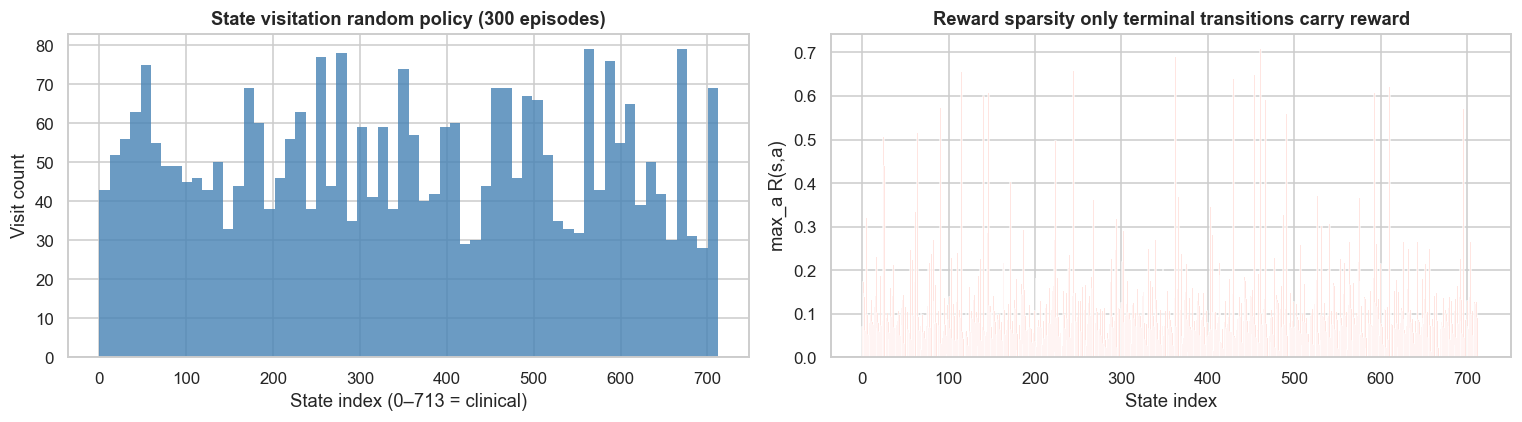
\includegraphics[width=\linewidth,height=0.18\textheight,keepaspectratio]{configA_env_exploration.png}
\caption{Config~A environment exploration.}
\label{fig:a_env}
\end{minipage}\hfill
\begin{minipage}{0.48\textwidth}
\centering
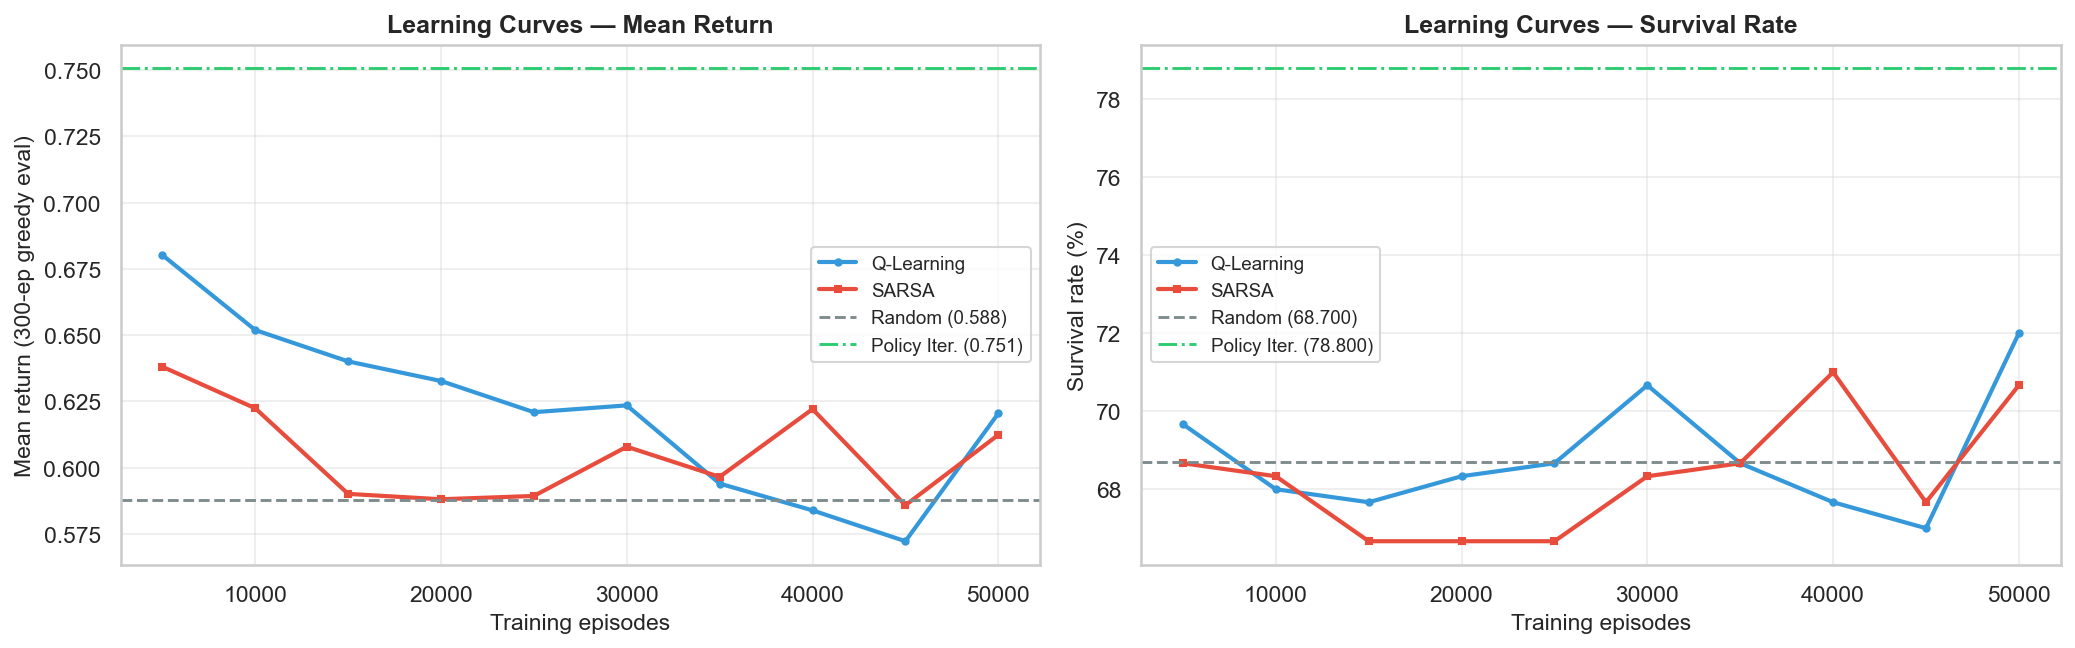
\includegraphics[width=\linewidth,height=0.18\textheight,keepaspectratio]{configA_learning_curves.png}
\caption{Config~A learning curves.}
\label{fig:a_learning}
\end{minipage}

\vspace{4pt}
\begin{minipage}{0.48\textwidth}
\centering
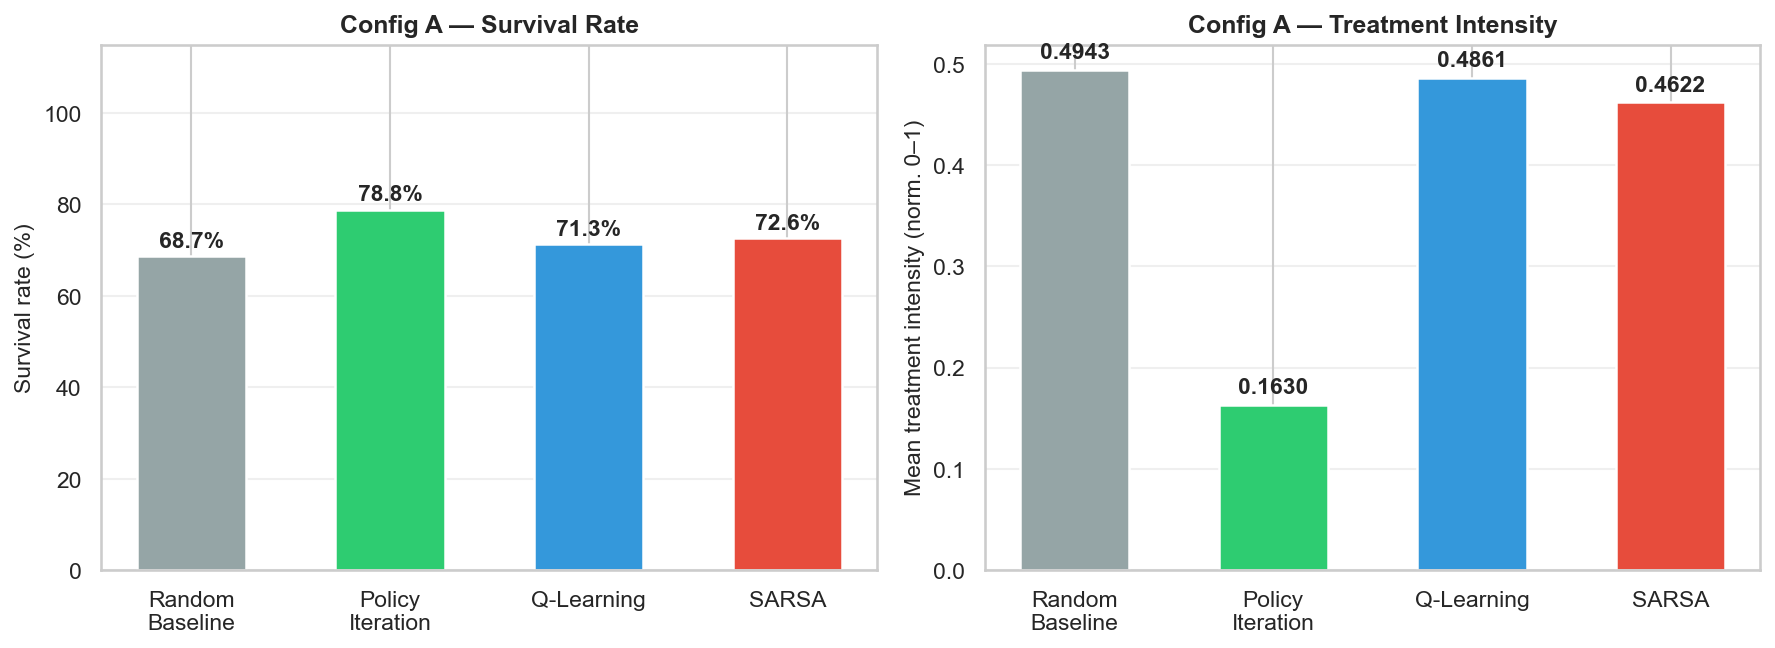
\includegraphics[width=\linewidth,height=0.18\textheight,keepaspectratio]{configA_survival_intensity.png}
\caption{Config~A survival and intensity.}
\label{fig:a_survint}
\end{minipage}\hfill
\begin{minipage}{0.48\textwidth}
\centering
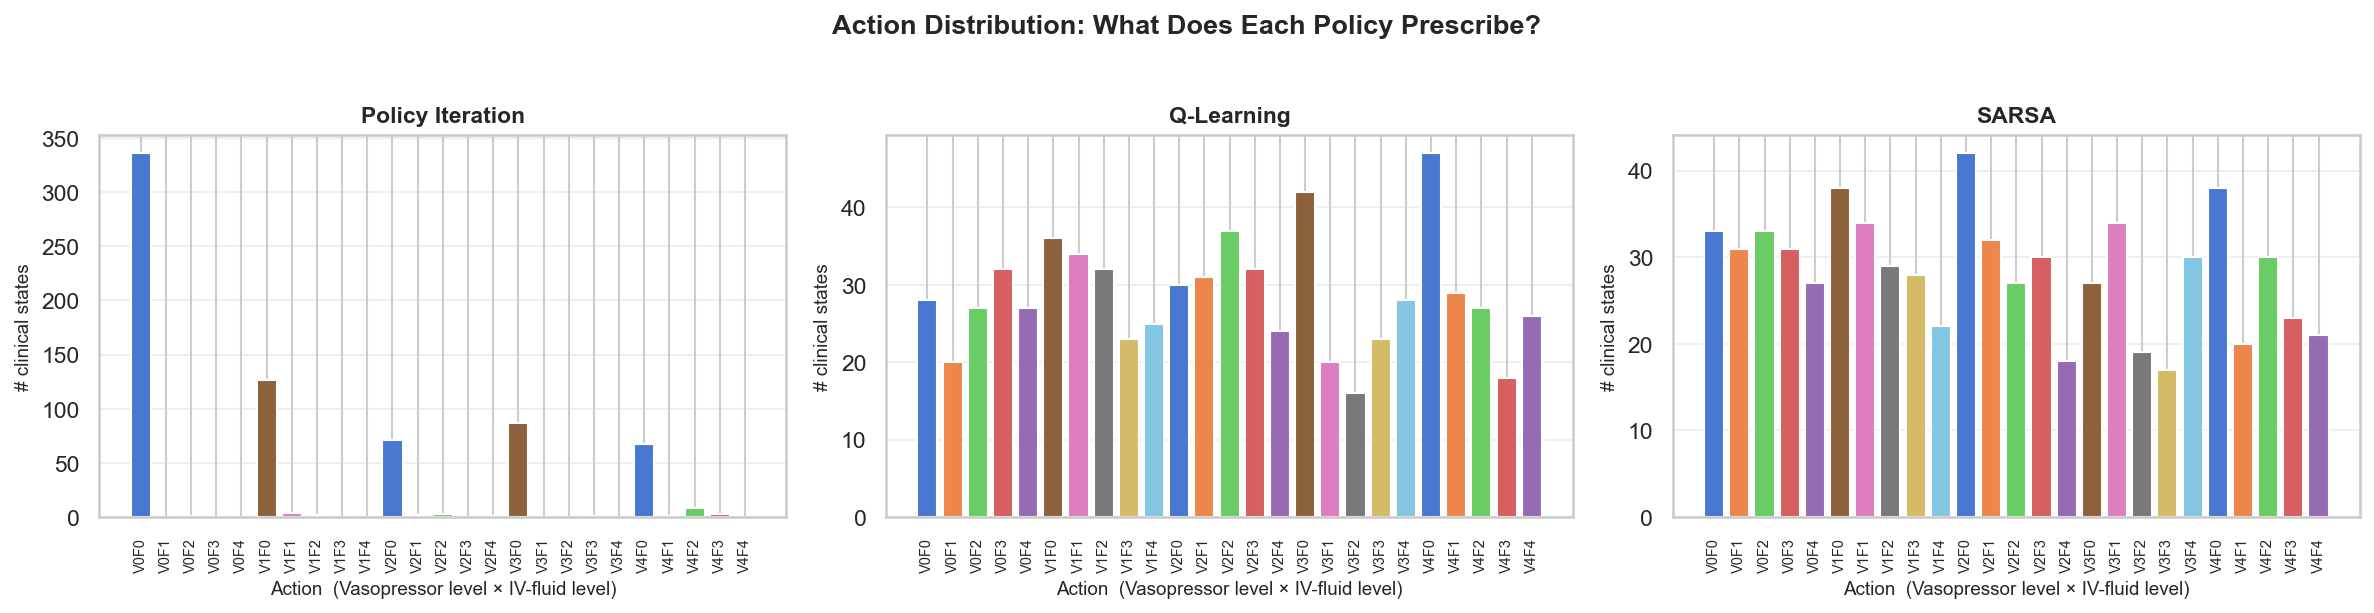
\includegraphics[width=\linewidth,height=0.18\textheight,keepaspectratio]{configA_action_distribution.png}
\caption{Config~A action distributions.}
\label{fig:a_actions}
\end{minipage}

\vspace{4pt}
\begin{minipage}{0.62\textwidth}
\centering
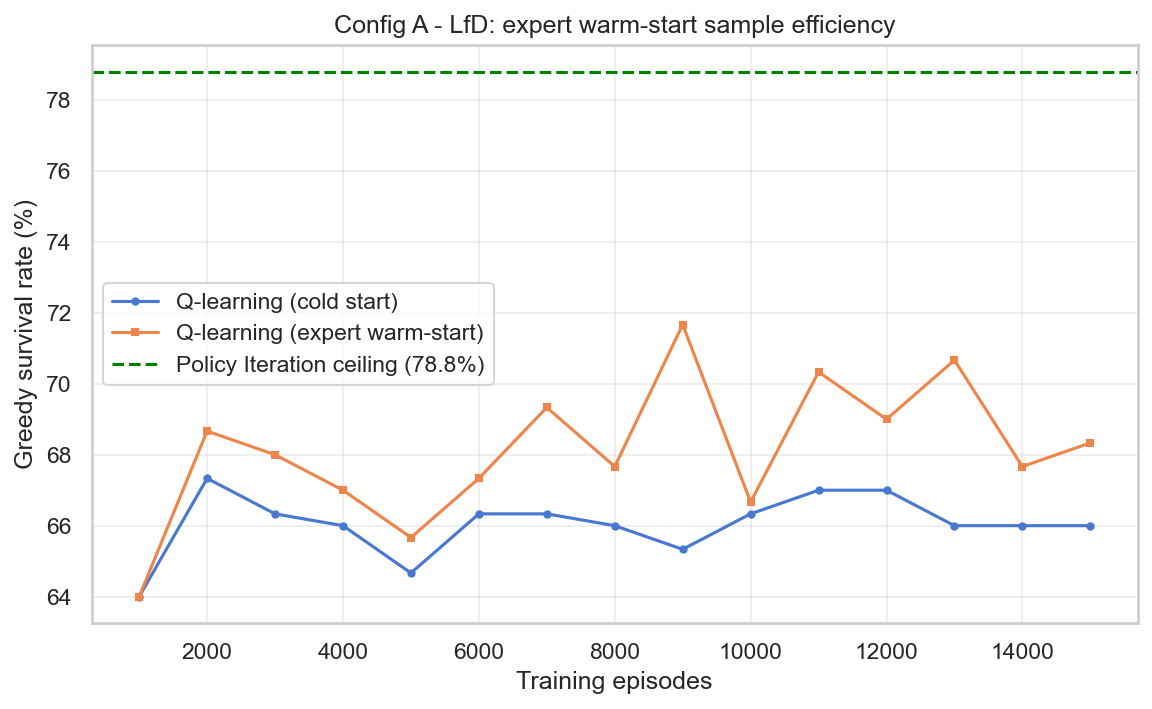
\includegraphics[width=\linewidth,height=0.18\textheight,keepaspectratio]{configA_warmstart.png}
\caption{Expert warm-start versus cold Q-Learning.}
\label{fig:a_warmstart}
\end{minipage}
\end{figure}

\subsection{Configuration~B}
\begin{figure}[H]
\centering
\begin{minipage}{0.48\textwidth}
\centering

\includegraphics[width=\linewidth,height=0.18\textheight,keepaspectratio]{configB_tuned_grid.png}
\caption{Tuned $1$M curves with linear trends.}
\label{fig:b_curves}
\end{minipage}\hfill
\begin{minipage}{0.48\textwidth}
\centering
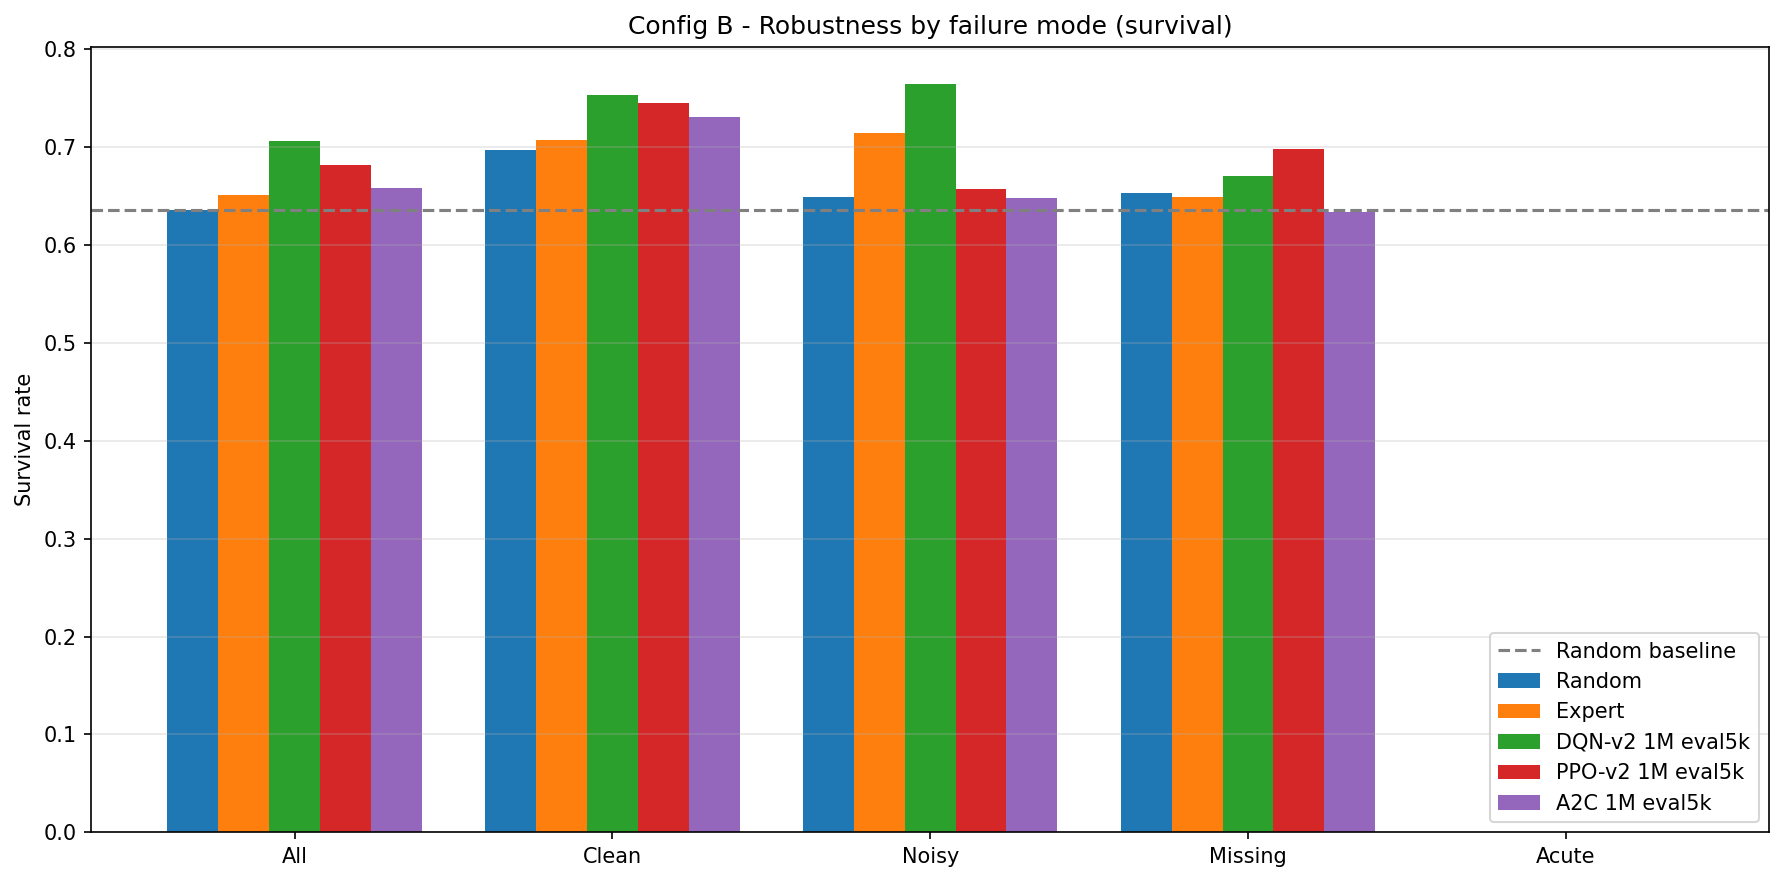
\includegraphics[width=\linewidth,height=0.18\textheight,keepaspectratio]{configB_1m_robustness_survival.png}
\caption{Config~B survival by failure mode.}
\label{fig:b_robust}
\end{minipage}

\vspace{4pt}
\begin{minipage}{0.48\textwidth}
\centering
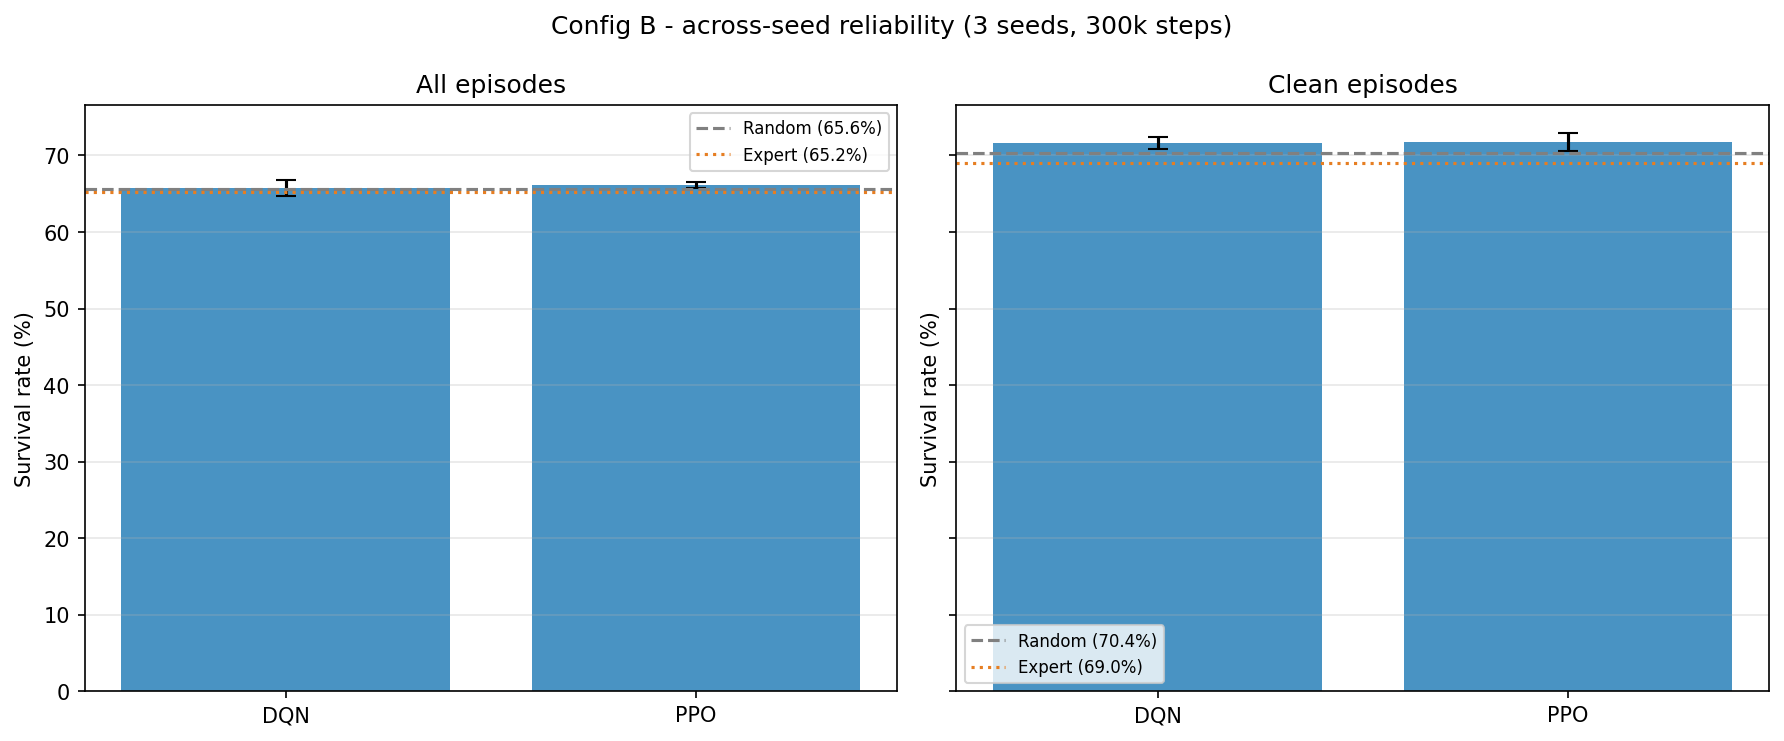
\includegraphics[width=\linewidth,height=0.18\textheight,keepaspectratio]{configB_multiseed.png}
\caption{Across-seed reliability.}
\label{fig:b_multiseed}
\end{minipage}\hfill
\begin{minipage}{0.48\textwidth}
\centering

\includegraphics[width=\linewidth,height=0.18\textheight,keepaspectratio]{configB_1m_dose_grid.png}
\caption{Learned vasopressor/fluid dose grids.}
\label{fig:b_dose}
\end{minipage}

\vspace{4pt}
\begin{minipage}{0.48\textwidth}
\centering
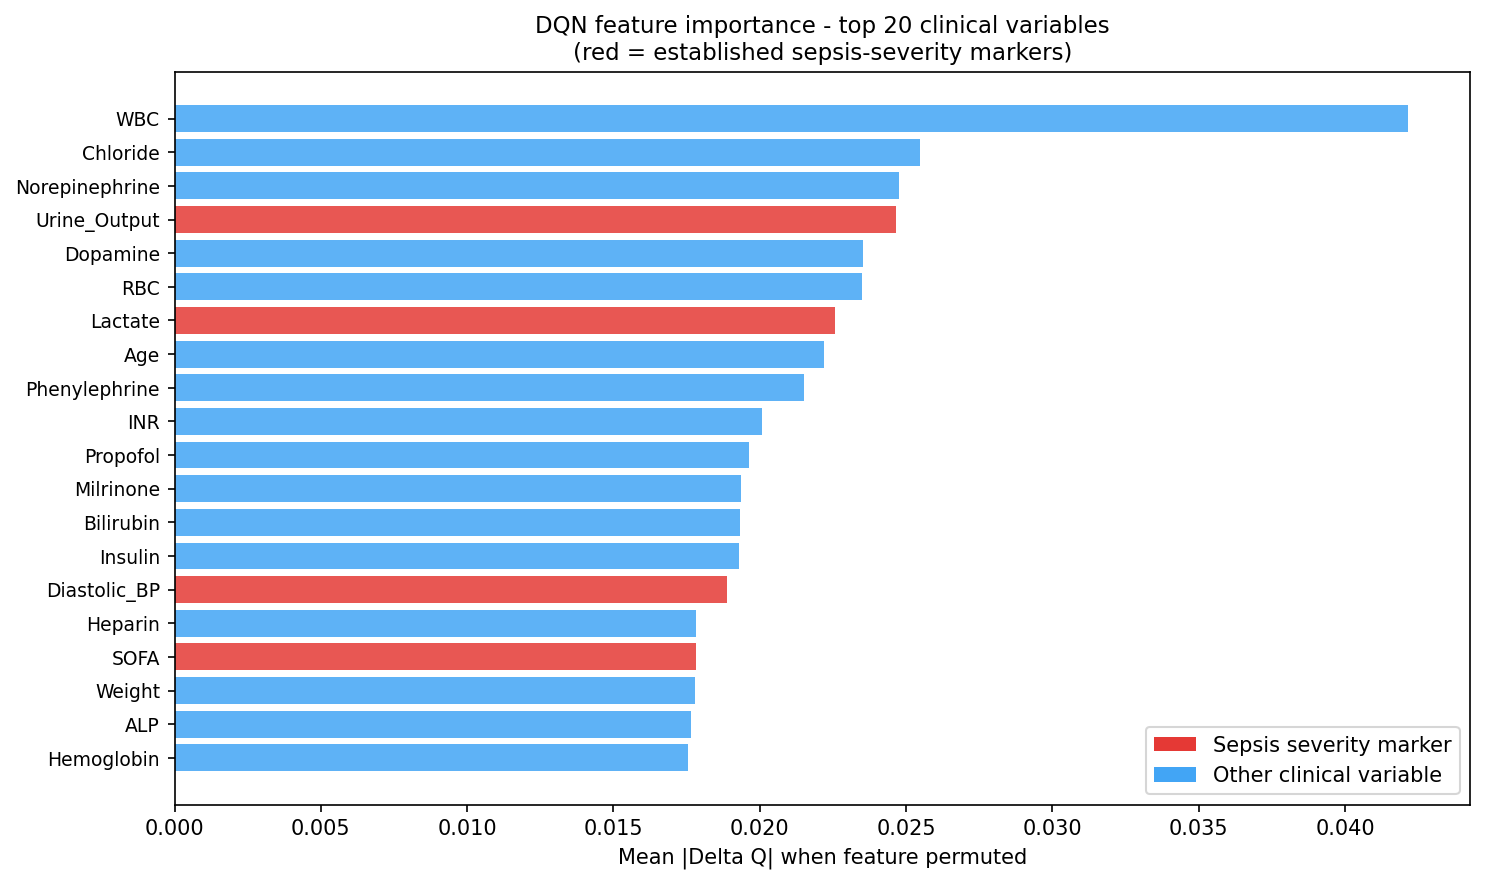
\includegraphics[width=\linewidth,height=0.18\textheight,keepaspectratio]{configB_1m_feature_importance.png}
\caption{DQN feature importance.}
\label{fig:b_feat}
\end{minipage}\hfill
\begin{minipage}{0.48\textwidth}
\centering
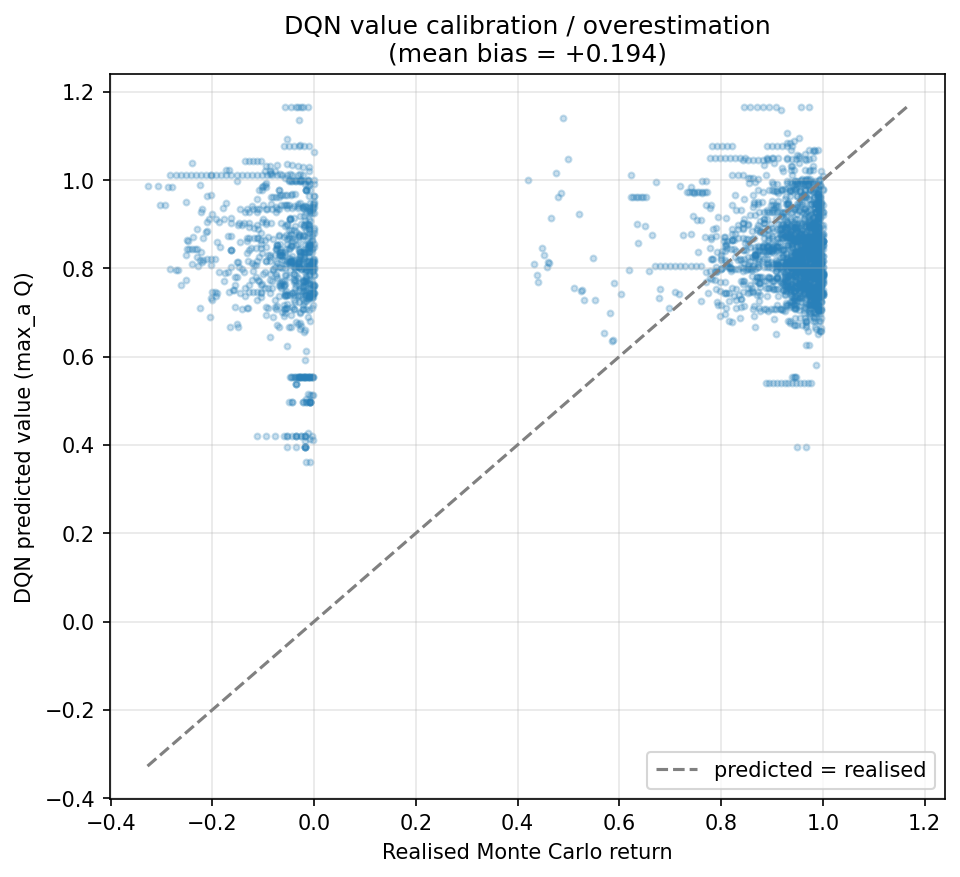
\includegraphics[width=\linewidth,height=0.18\textheight,keepaspectratio]{configB_overestimation.png}
\caption{DQN value overestimation diagnostic.}
\label{fig:b_overest}
\end{minipage}
\end{figure}

\endgroup

\end{document}
